\begin{minipage}{0.265\textwidth}
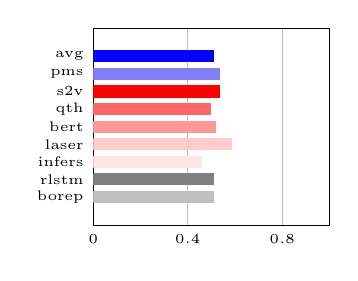
\begin{tikzpicture}

  	\begin{axis}[
 	   	xbar stacked,
		bar width=4pt,
		enlarge y limits=0.2,
    		symbolic y coords={borep,rlstm,infers,laser,bert,qth,s2v,pms,avg},
		xmin=0,xmax=1,
  		xmajorgrids,
		tickwidth=0pt,
		xtick distance=0.40,
  		ytick=data,
		scale only axis=true,
  		width=3cm,height=2.5cm,
		tick label style={font=\tiny}
  	]

		% avg
  		\addplot[blue,fill] coordinates
  			{(0.507,avg) (0.00,pms) (0.00,s2v) (0.00,qth) (0.00,bert) (0.00,laser) (0.00,infers) (0.00,rlstm) (0.000,borep)};
		% pms
		\addplot[blue!50,fill] coordinates
			{(0.00,avg) (0.534,pms) (0.00,s2v) (0.00,qth) (0.00,bert) (0.00,laser) (0.00,infers) (0.00,rlstm) (0.000,borep)};

		% s2v
		\addplot[red,fill] coordinates 
			{(0.00,avg) (0.00,pms) (0.534,s2v) (0.00,qth) (0.00,bert) (0.00,laser) (0.00,infers) (0.00,rlstm) (0.000,borep)};
		% qth
		\addplot[red!60,fill] coordinates
			{(0.00,avg) (0.00,pms) (0.00,s2v) (0.497,qth) (0.00,bert) (0.00,laser) (0.00,infers) (0.00,rlstm) (0.000,borep)};
		% bert
		\addplot[red!40,fill] coordinates
			{(0.00,avg) (0.00,pms) (0.00,s2v) (0.00,qth) (0.517,bert) (0.00,laser) (0.00,infers) (0.00,rlstm) (0.000,borep)};
		% laser
		\addplot[red!20,fill] coordinates
			{(0.00,avg) (0.00,pms) (0.00,s2v) (0.00,qth) (0.00,bert) (0.583,laser) (0.00,infers) (0.00,rlstm) (0.000,borep)};
		% infersent
		\addplot[red!10,fill] coordinates
			{(0.00,avg) (0.00,pms) (0.00,s2v) (0.00,qth) (0.00,bert) (0.00,laser) (0.456,infers) (0.00,rlstm) (0.000,borep)};

		% rand lstm
		\addplot[gray,fill] coordinates 
			{(0.00,avg) (0.00,pms) (0.00,s2v) (0.00,qth) (0.00,bert) (0.00,laser) (0.00,infers) (0.507,rlstm) (0.000,borep)};
		% borep
		\addplot[lightgray,fill] coordinates 
			{(0.00,avg) (0.00,pms) (0.00,s2v) (0.00,qth) (0.00,bert) (0.00,laser) (0.00,infers) (0.00,rlstm) (0.507,borep)};

  	\end{axis}

\end{tikzpicture}
\end{minipage}
\hfill
\begin{minipage}{0.25\textwidth}
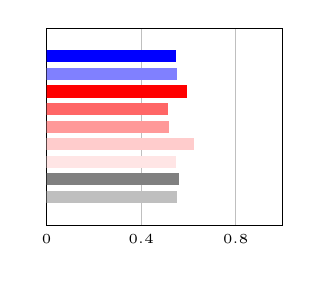
\begin{tikzpicture}

  	\begin{axis}[
   	 	xbar stacked,
		bar width=4pt,
		enlarge y limits=0.2,
	    	symbolic y coords={borep,rlstm,infers,laser,bert,qth,s2v,pms,avg},
		xmin=0,xmax=1,
  		xmajorgrids,
		tickwidth=0pt,
		xtick distance=0.40,
  		ytick=data,
		yticklabels={,,},
		scale only axis=true,
  		width=3cm,height=2.5cm,
		tick label style={font=\tiny}
  	]

		% avg
  		\addplot[blue,fill] coordinates
  			{(0.544,avg) (0.00,pms) (0.00,s2v) (0.00,qth) (0.00,bert) (0.00,laser) (0.00,infers) (0.00,rlstm) (0.000,borep)};
		% pms
		\addplot[blue!50,fill] coordinates
			{(0.00,avg) (0.550,pms) (0.00,s2v) (0.00,qth) (0.00,bert) (0.00,laser) (0.00,infers) (0.00,rlstm) (0.000,borep)};

		% s2v
		\addplot[red,fill] coordinates 
			{(0.00,avg) (0.00,pms) (0.590,s2v) (0.00,qth) (0.00,bert) (0.00,laser) (0.00,infers) (0.00,rlstm) (0.000,borep)};
		% qth
		\addplot[red!60,fill] coordinates
			{(0.00,avg) (0.00,pms) (0.00,s2v) (0.511,qth) (0.00,bert) (0.00,laser) (0.00,infers) (0.00,rlstm) (0.000,borep)};
		% bert
		\addplot[red!40,fill] coordinates
			{(0.00,avg) (0.00,pms) (0.00,s2v) (0.00,qth) (0.514,bert) (0.00,laser) (0.00,infers) (0.00,rlstm) (0.000,borep)};
		% laser
		\addplot[red!20,fill] coordinates
			{(0.00,avg) (0.00,pms) (0.00,s2v) (0.00,qth) (0.00,bert) (0.623,laser) (0.00,infers) (0.00,rlstm) (0.000,borep)};
		% infersent
		\addplot[red!10,fill] coordinates
			{(0.00,avg) (0.00,pms) (0.00,s2v) (0.00,qth) (0.00,bert) (0.00,laser) (0.547,infers) (0.00,rlstm) (0.000,borep)};

		% rand lstm
		\addplot[gray,fill] coordinates 
			{(0.00,avg) (0.00,pms) (0.00,s2v) (0.00,qth) (0.00,bert) (0.00,laser) (0.00,infers) (0.559,rlstm) (0.000,borep)};
		% borep
		\addplot[lightgray,fill] coordinates 
			{(0.00,avg) (0.00,pms) (0.00,s2v) (0.00,qth) (0.00,bert) (0.00,laser) (0.00,infers) (0.00,rlstm) (0.549,borep)};

  	\end{axis}

\end{tikzpicture}
\end{minipage}
\hfill
\begin{minipage}{0.25\textwidth}
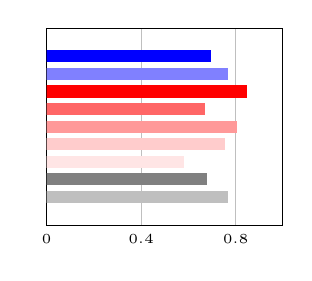
\begin{tikzpicture}

  	\begin{axis}[
 	   	xbar stacked,
		bar width=4pt,
		enlarge y limits=0.2,
    		symbolic y coords={borep,rlstm,infers,laser,bert,qth,s2v,pms,avg},
		xmin=0,xmax=1,
  		xmajorgrids,
		tickwidth=0pt,
		xtick distance=0.40,
  		ytick=data,
		yticklabels={,,},
		scale only axis=true,
  		width=3cm,height=2.5cm,
		tick label style={font=\tiny}
  	]

		% avg
  		\addplot[blue,fill] coordinates
  			{(0.694,avg) (0.00,pms) (0.00,s2v) (0.00,qth) (0.00,bert) (0.00,laser) (0.00,infers) (0.00,rlstm) (0.000,borep)};
		% pms
		\addplot[blue!50,fill] coordinates
			{(0.00,avg) (0.765,pms) (0.00,s2v) (0.00,qth) (0.00,bert) (0.00,laser) (0.00,infers) (0.00,rlstm) (0.000,borep)};

		% s2v
		\addplot[red,fill] coordinates 
			{(0.00,avg) (0.00,pms) (0.846,s2v) (0.00,qth) (0.00,bert) (0.00,laser) (0.00,infers) (0.00,rlstm) (0.000,borep)};
		% qth
		\addplot[red!60,fill] coordinates
			{(0.00,avg) (0.00,pms) (0.00,s2v) (0.667,qth) (0.00,bert) (0.00,laser) (0.00,infers) (0.00,rlstm) (0.000,borep)};
		% bert
		\addplot[red!40,fill] coordinates
			{(0.00,avg) (0.00,pms) (0.00,s2v) (0.00,qth) (0.802,bert) (0.00,laser) (0.00,infers) (0.00,rlstm) (0.000,borep)};
		% laser
		\addplot[red!20,fill] coordinates
			{(0.00,avg) (0.00,pms) (0.00,s2v) (0.00,qth) (0.00,bert) (0.753,laser) (0.00,infers) (0.00,rlstm) (0.000,borep)};
		% infersent
		\addplot[red!10,fill] coordinates
			{(0.00,avg) (0.00,pms) (0.00,s2v) (0.00,qth) (0.00,bert) (0.00,laser) (0.580,infers) (0.00,rlstm) (0.000,borep)};

		% rand lstm
		\addplot[gray,fill] coordinates 
			{(0.00,avg) (0.00,pms) (0.00,s2v) (0.00,qth) (0.00,bert) (0.00,laser) (0.00,infers) (0.676,rlstm) (0.000,borep)};
		% borep
		\addplot[lightgray,fill] coordinates 
			{(0.00,avg) (0.00,pms) (0.00,s2v) (0.00,qth) (0.00,bert) (0.00,laser) (0.00,infers) (0.00,rlstm) (0.764,borep)};

  	\end{axis}

\end{tikzpicture}
\end{minipage}
%\hfill
%\begin{minipage}{0.1\textwidth}
%\begin{tikzpicture}
%
%  	\begin{axis}[
% 	   	xbar stacked,
%		bar width=4pt,
%		enlarge y limits=0.2,
%    		symbolic y coords={rlstm,infers,laser,bert,qth,s2v,pms,avg},
%		xmin=0,xmax=1,
%  		xmajorgrids,
%		tickwidth=0pt,
%		xtick distance=0.40,
%  		ytick=data,
%		yticklabels={,,},
%		scale only axis=true,
%  		width=1.3cm,height=2cm,
%		tick label style={font=\tiny}
%  	]
%
%		% avg
%  		\addplot[blue,fill] coordinates
%  			{(0.884,avg) (0.00,pms) (0.00,s2v) (0.00,qth) (0.00,bert) (0.00,laser) (0.00,infers) (0.00,rlstm)};
%		% pms
%		\addplot[blue!50,fill] coordinates
%			{(0.00,avg) (0.873,pms) (0.00,s2v) (0.00,qth) (0.00,bert) (0.00,laser) (0.00,infers) (0.00,rlstm)};
%
%		% s2v
%		\addplot[red,fill] coordinates 
%			{(0.00,avg) (0.00,pms) (0.867,s2v) (0.00,qth) (0.00,bert) (0.00,laser) (0.00,infers) (0.00,rlstm)};
%		% qth
%		\addplot[red!60,fill] coordinates
%			{(0.00,avg) (0.00,pms) (0.00,s2v) (0.831,qth) (0.00,bert) (0.00,laser) (0.00,infers) (0.00,rlstm)};
%		% bert
%		\addplot[red!40,fill] coordinates
%			{(0.00,avg) (0.00,pms) (0.00,s2v) (0.00,qth) (0.876,bert) (0.00,laser) (0.00,infers) (0.00,rlstm)};
%		% laser
%		\addplot[red!20,fill] coordinates
%			{(0.00,avg) (0.00,pms) (0.00,s2v) (0.00,qth) (0.00,bert) (0.906,laser) (0.00,infers) (0.00,rlstm)};
%		% infersent
%		\addplot[red!10,fill] coordinates
%			{(0.00,avg) (0.00,pms) (0.00,s2v) (0.00,qth) (0.00,bert) (0.00,laser) (0.875,infers) (0.00,rlstm)};
%
%		% rand lstm
%		\addplot[gray,fill] coordinates 
%			{(0.00,avg) (0.00,pms) (0.00,s2v) (0.00,qth) (0.00,bert) (0.00,laser) (0.00,infers) (0.874,rlstm)};
%
%  	\end{axis}
%
%\end{tikzpicture}
%\end{minipage}
%\hfill
%\begin{minipage}{0.1\textwidth}
%\begin{tikzpicture}
%
%  	\begin{axis}[
%   	 	xbar stacked,
%		bar width=4pt,
%		enlarge y limits=0.2,
%	    	symbolic y coords={rlstm,infers,laser,bert,qth,s2v,pms,avg},
%		xmin=0,xmax=1,
%  		xmajorgrids,
%		tickwidth=0pt,
%		xtick distance=0.40,
%  		ytick=data,
%		yticklabels={,,},
%		scale only axis=true,
%  		width=1.3cm,height=2cm,
%		tick label style={font=\tiny}
%  	]
%
%		% avg
%  		\addplot[blue,fill] coordinates
%  			{(0.00,avg) (0.00,pms) (0.00,s2v) (0.00,qth) (0.00,bert) (0.00,laser) (0.00,infers) (0.00,rlstm)};
%		% pms
%		\addplot[blue!50,fill] coordinates
%			{(0.00,avg) (0.00,pms) (0.00,s2v) (0.00,qth) (0.00,bert) (0.00,laser) (0.00,infers) (0.00,rlstm)};
%
%		% s2v
%		\addplot[red,fill] coordinates 
%			{(0.00,avg) (0.00,pms) (0.00,s2v) (0.00,qth) (0.00,bert) (0.00,laser) (0.00,infers) (0.00,rlstm)};
%		% qth
%		\addplot[red!60,fill] coordinates
%			{(0.00,avg) (0.00,pms) (0.00,s2v) (0.00,qth) (0.00,bert) (0.00,laser) (0.00,infers) (0.00,rlstm)};
%		% bert
%		\addplot[red!40,fill] coordinates
%			{(0.00,avg) (0.00,pms) (0.00,s2v) (0.00,qth) (0.00,bert) (0.00,laser) (0.00,infers) (0.00,rlstm)};
%		% laser
%		\addplot[red!20,fill] coordinates
%			{(0.00,avg) (0.00,pms) (0.00,s2v) (0.00,qth) (0.00,bert) (0.00,laser) (0.00,infers) (0.00,rlstm)};
%
%		% rand lstm
%		\addplot[gray,fill] coordinates 
%			{(0.00,avg) (0.00,pms) (0.00,s2v) (0.00,qth) (0.00,bert) (0.00,laser) (0.00,infers) (0.00,rlstm)};
%
%  	\end{axis}
%
%\end{tikzpicture}
%\end{minipage}
%\hfill
%\begin{minipage}{0.1\textwidth}
%\begin{center}
%\textit{n.\,a.}
%\end{center}
%\end{minipage}
%\hfill
%\begin{minipage}{0.1\textwidth}
%\begin{center}
%\textit{n.\,a.}
%\end{center}
%\end{minipage}
%\hfill
%\begin{minipage}{0.1\textwidth}
%\begin{center}
%\textit{n.\,a.}
%\end{center}
%\end{minipage}